\documentclass[10pt,a4paper]{report}
%\usepackage[latin1]{inputenc}
\usepackage[utf8]{inputenc}
\usepackage{amsmath}
\usepackage{amsfonts}
\usepackage{amssymb}
\usepackage{graphicx}
\usepackage{multicol}
\usepackage{tabularx}
\usepackage{tikz}
\usetikzlibrary{arrows,shapes,automata,petri,positioning,calc}
\usepackage{hyperref}
\usepackage{tikz}
\usetikzlibrary{matrix,calc}
\usepackage[margin=0.5in]{geometry}
% ---- power functions -----% 
\newcommand{\myvec}[1]{\ensuremath{\begin{pmatrix}#1\end{pmatrix}}}
\let\vec\mathbf

\providecommand{\norm}[1]{\left\lVert#1\right\rVert}
\providecommand{\abs}[1]{\left\vert#1\right\vert}
\let\vec\mathbf

\newcommand{\mydet}[1]{\ensuremath{\begin{vmatrix}#1\end{vmatrix}}}
\providecommand{\brak}[1]{\ensuremath{\left(#1\right)}}
\providecommand{\lbrak}[1]{\ensuremath{\left(#1\right.}}
\providecommand{\rbrak}[1]{\ensuremath{\left.#1\right)}}
\providecommand{\sbrak}[1]{\ensuremath{{}\left[#1\right]}}
%-------end power functions----%
\newenvironment{Figure}
  {\par\medskip\noindent\minipage{\linewidth}}
  {\endminipage\par\medskip}
\begin{document}
%--------------------logo figure-------------------------%
\begin{figure*}[!tbp]
  \centering
  \begin{minipage}[b]{0.4\textwidth}
    
\includegraphics[scale = 0.05]{iitlogo.jpg}
  \end{minipage}
  \hfill
  \vspace{5mm}\begin{minipage}[b]{0.4\textwidth}
\raggedleft  
\includegraphics[scale = 0.10]{nrc.png}\

  \end{minipage}\vspace{0.2cm}
\end{figure*}
%--------------------name & rollno-----------------------
\raggedright \textbf{Name}:\hspace{1mm} V.Meghana \hspace{3cm} \Large \textbf{Assignment-5}\hspace{2.5cm} % 
\normalsize \textbf{Roll No.} :\hspace{1mm} FWC22045\vspace{1cm}
\begin{multicols}{2}

%----------------problem statement--------------%
\raggedright \section{Problem Statement:}%\vspace{2mm}
\raggedright
 If the lines 2x+3y+1 =0 and 3x-y-4 = 0 lie along diameter of a circle of circumference $10\pi$, then the equation of the circle is. \\
\vspace{5mm}
%-----------------------------solution---------------------------
\raggedright \section{SOLUTION:}\vspace{2mm}

%---------given----------------%
\raggedright \textbf{Given}:\vspace{2mm}\\
Two line equations are \\\vspace{1mm}
\begin{align}
\vspace{1mm}
\vec{n_1}^\top\textbf{x}={c_1}
\\
\vec{n_2}^\top\textbf{x}={c_2}
\end{align}
Above two equations are diameters of the circle.\\ \vspace{1mm}
We know that the diameters intersect at the \textbf{centre} of the circle.\\
So solving those two equations, we get the centre of the circle.
\\
Let \textbf{x} be the centre of the circle.
\begin{align}
 \textbf{x} = 
 \myvec{
\vec{n_1} \hspace{2mm} \vec{n_2} \\
}^{-\top}\vec{c}
\end{align}
where,
\begin{align}
\vec{n_1}=\myvec{2 \\ 3} ,\vec{n_2}=\myvec{3 \\-1} \textbf{c}=\myvec{-1 \\4}
\\
 \textbf{x} =
 \myvec{
2 \hspace{3mm} 3 \\
3 \hspace{3mm} -1 \\
}^{-\top}
\myvec{
      -1\\
      4
  }
\end{align}

%-------------To find ------------------%
\textbf{To Find }\vspace{2mm}\\
We can find the centre of the circle by solving the above equation through finding the inverse \vspace{2mm}  \\ 
From the above equation we get the centre of the circle i.e, \\\vspace{1mm}
\begin{align}
    \vec{x} =
    \myvec{
    1\\
    -1
    }
\end{align}
\textbf{STEP-1}\vspace{2mm}\\
Given that the Circumference of the circle is 10$\pi$. \\ \vspace{1mm}
\begin{align}
    2\pi{r} = 10\pi
    \\ \vspace{1mm}
    \\
    {r} = 5
\end{align}

\textbf{STEP-2}\vspace{2mm}\\
The general equation of the circle is given by,\\ \vspace{1mm}
\begin{align}
    \textbf{X}^\top \textbf{V}\textbf{X}+2\textbf{u}^\top\textbf{X}+{f} = 0
\end{align}
\\
where, \\ \vspace{1mm}
\begin{align}
    f = \vec{\norm{u}}^2-{r}^2\\
    \vec{V}=\vec{I}=\myvec{
    1 \hspace{4mm} 0 \\ \vspace{1mm}
    0 \hspace{4mm} 1 \
    }
    \\ \vspace{1mm}
    \textbf{u}=\myvec{
    {-1}
    \\
    {1}
    }
\end{align}
Substituting all the values in the above equation, we get \\

\begin{align}
    \textbf{X}^\top \myvec{
    1 \hspace{4mm} 0 \\ \vspace{1mm}
    0 \hspace{4mm} 1 \
    }
    \textbf{x}+2\myvec{
    -1
    \hspace{4mm}
    1
    }\textbf{X} - 23 = 0
\end{align}

\section{Construction}
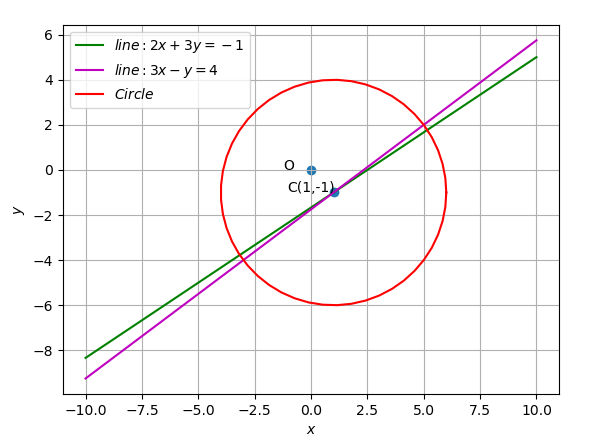
\includegraphics[scale=0.35]{circle.png}  

%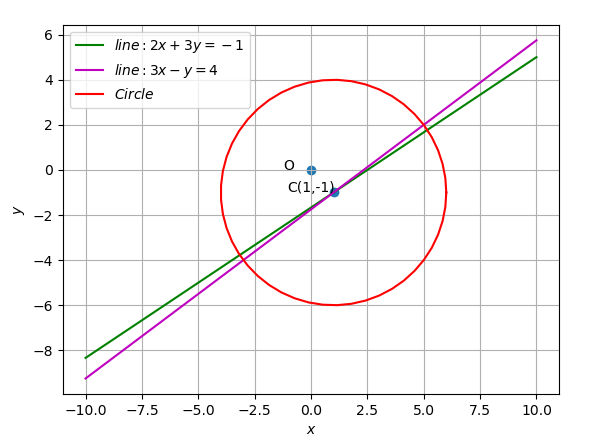
\includegraphics[width=0.5\textwidth]{circle.png}  
 %\end{center}
 \textbf{Download the code} \\
Github link:{https://github.com/Meghana9121/FWC}.
  \end{multicols}
\end{document}
